\chapter{Team 1 Agent Design}\label{team_1_agent_design}

\section{Overview}

The following chapter presents the design and implementation of Team 1's agent. The presented agent seeks to imitate important parts of human behaviour such as social status, social networks, selfishness, forgiveness and learning from experience. At the end of the chapter, it will be shown that by using these concepts, the agent produces better collective outcomes over agents performing random actions.

\section{Core Structure}
Figure \ref{fig:agent_structure} presents a high-level overview of the structure and operation of our agent. In broad terms, the agent contains three elements which impact decision-making. These elements are:    
\begin{enumerate}
  \item Social capital: Socially constructed resources which facilitate cooperation to solve collective problems.
  \item Selfishness: A continuously updated variable dictating to what degree an  agent prioritizes its own utility over the social welfare of the group when making decisions. 
  \item Q-functions: Functions learned through reinforcement learning which estimate the impact of actions given the current game state.
\end{enumerate}
In addition to these components which are inherent to the agent, the current state of the game, known as the \emph{environment}, also influences decisions. Exactly how each component is used in the decision making process varies between different types of decisions, and social capital, selfishness and Q-functions are not all used for every decision. The specific decision process for each type of decision will be discussed in greater detail later on.

%However, a general decision flow can be as follows: The agent takes in the current game state and passes it through a set of Q-functions. The Q-functions return the expected utility of each action to the collective and to the agent itself. Based on its current selfishness value, the agent aggregates the two utility values into a single value for each action.   Generally, the decision flow 

After each round of the game, the agents will update their internal state. Specifically, the agents will update their selfishness based on the current environment and the social capital of agents, while the social capital will be updated based on the actions of agents. The social capital is also updated every time an agent receives a message from an agent in their network. All of these update mechanisms are indicated by red arrows in Figure \ref{fig:agent_structure}. As can be seen, there is no arrow feeding back to the Q-functions as they do not update over the course of a single game. Instead, the Q-functions are updated based on the results from a series of games. However, as will be discussed later, the updating of selfishness values does still permit the agents to learn from experiences during a game.

% In addition to selfishness and social capital the agent also maintains a set of state variables that are used to make decisions with regard to leadership and voting. The most important of these is a measure of how well each agent in currently doing. This variable has to take into account many different aspects of game state and can be fairly difficult to create as defining a good game position is not obvious and of course depends on the decisions of others. An example of this difficulty is in deciding whether or not an agent having a higher attack value suggests it is doing better, in this case we found this to be a bad thing as in makes the agent more likely to have to engage in fights compared to agents with lower attacks. Several different factors such as this were combined to form this single variable which will be referred to as agent survival likelihood from here on. Once this score was computed for each agent all the scores were scaled such that the maximum score was less than 1 and the minimum was greater that 0, in addition, the mean was shifted so as to be close to 0.5. Finally, the standard deviation of this data-set was computed to give an indication of the spread of agents states, as the variation in state across the population can be a big factor in agent decision making. 

\begin{figure}[!h]
    \centering
    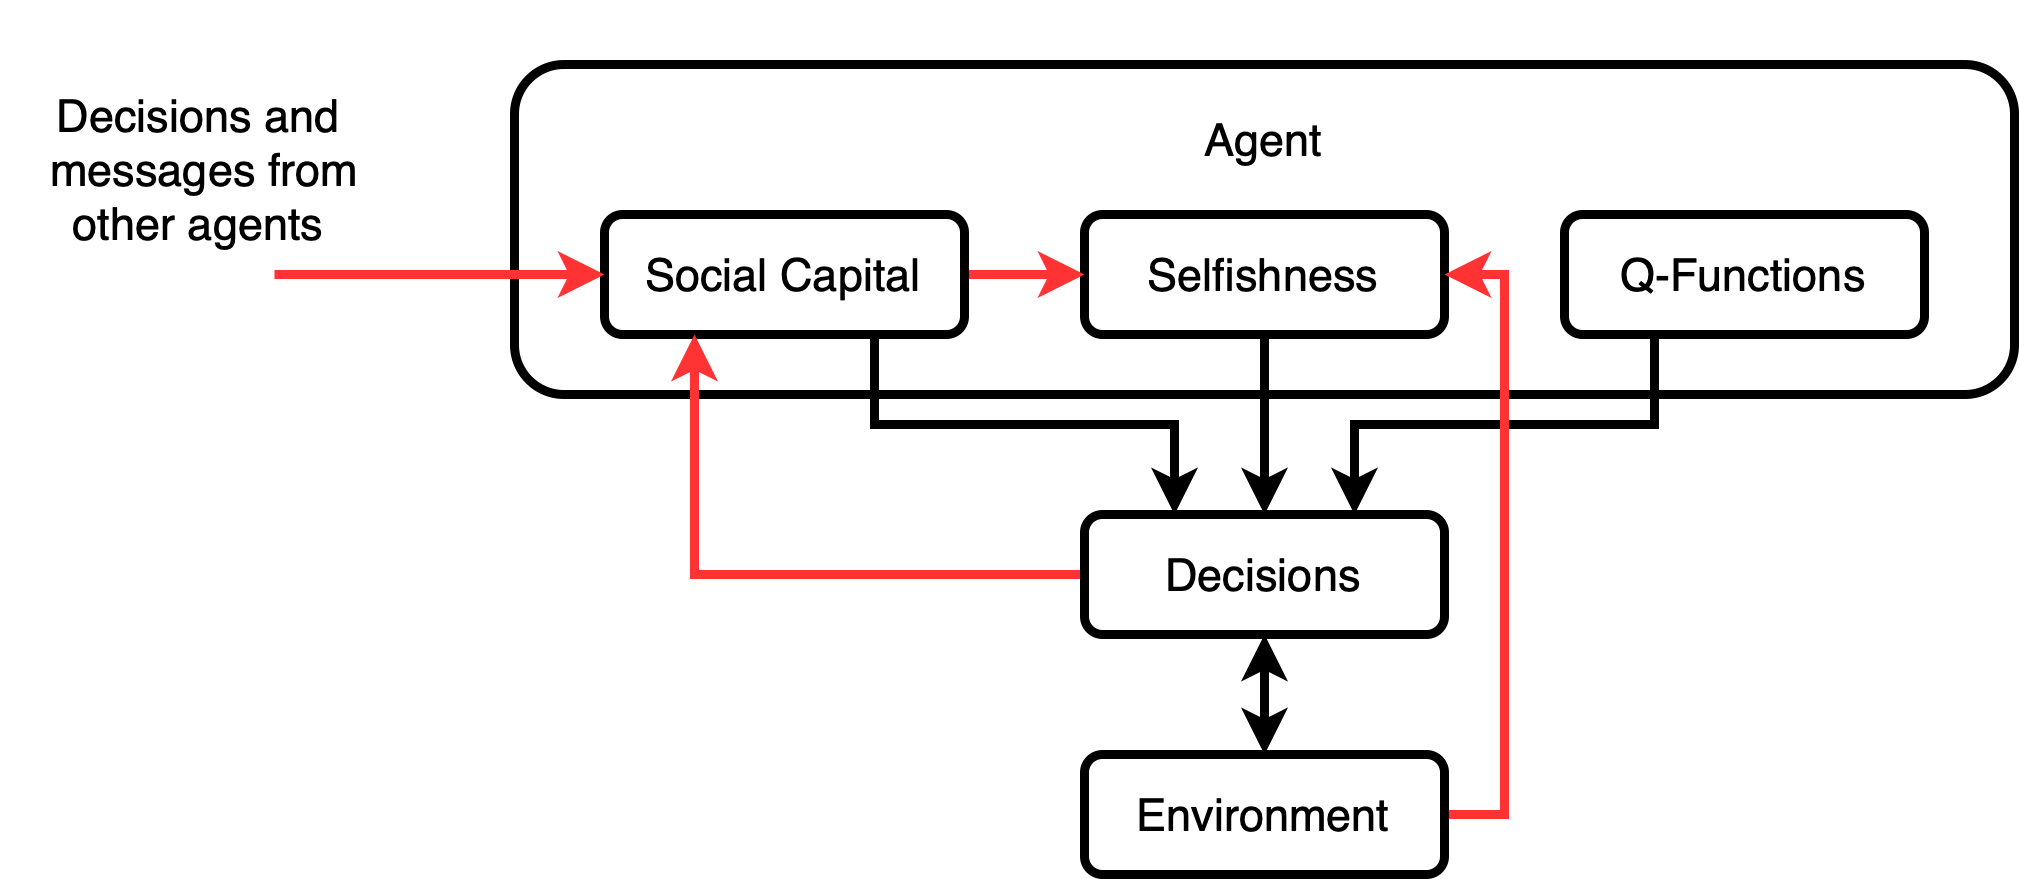
\includegraphics[width=0.75\linewidth]{004_team_1_agent_design/images/agent_structure.png}
    \caption{Overview of agent structure.}
    \label{fig:agent_structure}
\end{figure}

\section{Social Capital}

The core concept underlying the design of the agent is the idea of social capital. The exact definition of the term "social capital" varies between works, but can be summarized as "an 'umbrella term' for a range of socially constructed conceptual resources that help people coordinate expectations and self-organise."\cite{pitt}. Several forms of social capital have been identified and defined. Our work on social capital is mostly related to those forms laid out by Elinor Ostrom and T. K. Ahn in their 2007 paper "The meaning of social capital and its link to collective action". \cite{ostrom-ahn} In their paper, Ostrom and Ahn identified three forms of social capital. These were \emph{Institutions}, \emph{Networks} and \emph{Trustworthiness}. In addition to the forms of social capital presented by Ostrom and Ahn, we have as a team identified another form of social capital we call \emph{Honour}. With \emph{Honour} we refer to the human tendency to want to return a favour, or similarly, our appetite for revenge. A more comprehensive definition of honour is given in section \ref{subsection:honour}. 

In order to use social capital to promote cooperation, it must be used as part of a framework where the actions of an agent impact their social capital and where the social capital is used to make informed decision on whether or not to cooperate with other agents. For our agent, we used a similar framework to that presented by Petruzzi, Pitt, and Busquets\cite{complexity_reduction}. An overview diagram of this framework is presented in Figure \ref{fig:social_capital_framework}. In this framework, events coming from the environment are translated into social capital information which is passed to internal update functions for calculating metrics for each type of social capital. The social capital decision module uses the social capital metrics to calculate a value from 0 (no cooperation) to 1 (full cooperation) indicating whether an agent should cooperate or not. Implementing this framework for a simple cooperation game, Petruzzi et al. were able to achieve better performance than the dominant strategy given by game theory analysis. 

\begin{figure}[!h]
    \centering
    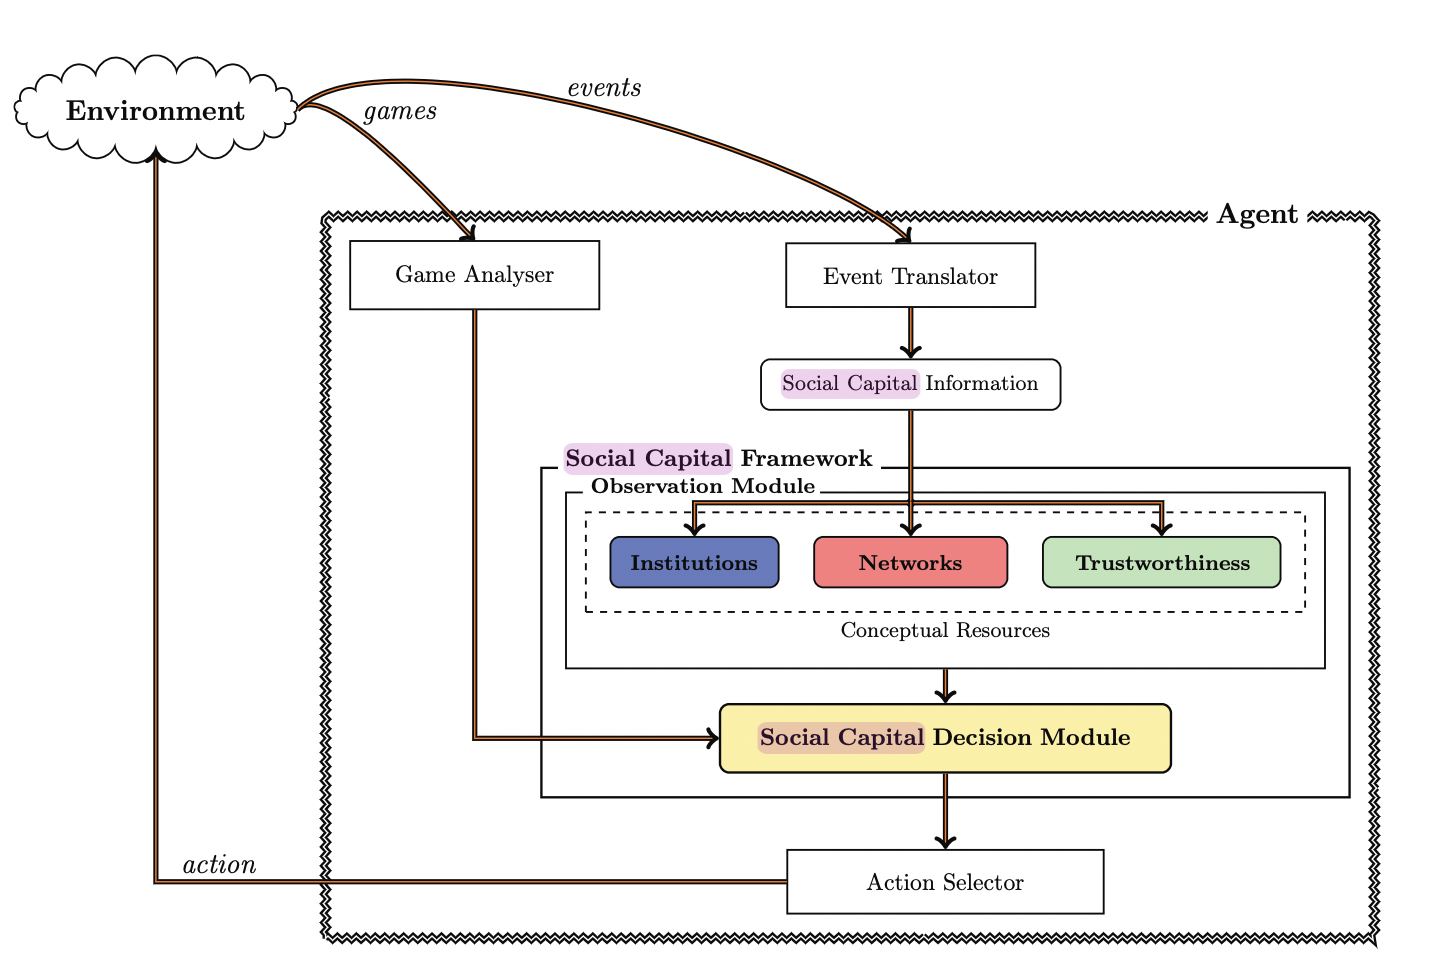
\includegraphics[width=0.75\linewidth]{004_team_1_agent_design/images/socialcapitalframework.png}
    \caption{Framework for a social capital system.\cite{pitt}}
    \label{fig:social_capital_framework}
\end{figure}

To apply the framework to the Escape the Dark Pit(t) game, we used a slightly different implementation than Petruzzi et al. used for their cooperation game. Most prominently, we simplified the stored metrics on social capital down to a single number between -1 and 1 for each form of social capital. We also simplified the social capital decision module by removing the possibility of weighting social capital indicators differently, reducing the decision module to a simple summing function. 

The specific implementation is as follows. Each agent has a member variable $socialCapital$ which is a map between agent ids and an array with 4 values. From index 0 to index 3, this array holds values describing the social capital related to institutions, networks, trustworthiness and honour respectively for the agent with the specified agent id. Each agents $socialCapital$ map contains an array for every single agent in the game, including themselves. The array values are bounded between -1 and 1, where a higher number indicates higher social capital. When an agent is created, all the array values are initialized as 0. This is a neutral state in which no agent has a negative nor positive impression of another agent. Throughout the game the array values for each agent will change based on their actions and messages received about them. In general, if an agent does a non-cooperative actions the array values will decrease and become negative, and inversely, cooperative actions will give positive array values. As such, agents will try to reward other agents when their $socialCapital$ map indicates positive social capital and punish those who have negative social capital.

The following subsections go into detail regarding the implementation of each form of social capital.

\subsection{Institutions}

In their 2007 paper Ostrom and Ahn defined institutions as "prescriptions that specify what actions (or outcomes) are required, prohibited, or permitted, and the sanctions authorized if the rules are not followed" \cite{ostrom-ahn}. With our $Institutions$ social capital value we seek to provide a metric on how likely an agent is to follow these prescriptions and cooperate within institutions. 

During a game our agents place the following expectation on the interaction of other agents with institutions:

\begin{enumerate}
    \item If the leader makes a fight proposal, all agents should follow that proposal.
    \item If the leader makes a loot allocation proposal, all agents should follow that proposal.
\end{enumerate}

Failing to comply with any of these two expectations will lead to an agent being labelled as a defector. Once labelled as a defector, an agent's social capital value for institutions will for the rest of the game be given a base value of -1. As such, even deviating from the required action once will lead to a negative perception for the entirety of the remaining game. This is similar to a grim trigger strategy for cooperation. The reason why we elected to have defecting in even a single round negatively affect the social capital of an agent for all remaining rounds is due to the limitation on available information from the game. In its current version, the list of defectors which the game makes available to the agent has the same type of static behaviour where defecting once will lead to an agent being labelled as a defector for the rest of the game.

In order to increase their $Institutions$ social capital value agents must demonstrate their cooperation within institutions. For our agents there is just a single way of doing this: being elected leader. For as long as an agent is the leader, they will get a temporary boost of +1 to their $Institutions$ social capital value. Originally, the tendency for agents to sanction defectors was also planned to impact their social capital. In this case, doing actions which punish defectors such as voting against them in elections and not trading with them would yield positive social capital. Inversely, voting for defectors or trading with them would yield negative social capital. However, this was in practice found to be hard to implement, and has been left as a possible future extension.

\subsection{Networks}
The $Networks$ social capital value is a measure of an agent's reputation among other agents. Specifically, the $Networks$ value tries to estimate the average social capital perception of the given agent among the other agents in the game. The $Networks$ value is also used by agents in order to determine which other agents they want to share social capital information with. This way, agents will form a social network in which each agent is liked by the other agents in its network.

In our current configuration, an agent will communicate with other agents if they have a social capital $Networks$ value greater or equal to $T_{N_0} = 0.5$. Previously, we have said that all social capital values are initialized to zero. This is a slight oversimplification, as we in fact initialise a small subset of $Networks$ values for each agent to 0.8. This was necessary given the way an agent decides whether to communicate with other agents, as agents would never communicate if $Networks$ values were all zero and thus the $Networks$ values would never update. 

We investigated several ways of determining what $Networks$ values to give a non-zero initialization and thus which other agents an agent should communicate with from the beginning. For example, agents can be initialised in a grid structure (figure \ref{fig:sc_network_grid}) where most agents are connected to four other agents, aside from agents at the edges or corners that are only connected to three or two agents respectively. This is the initialisation structure our agents currently use.

% \begin{figure}[!h]
%     \centering
%     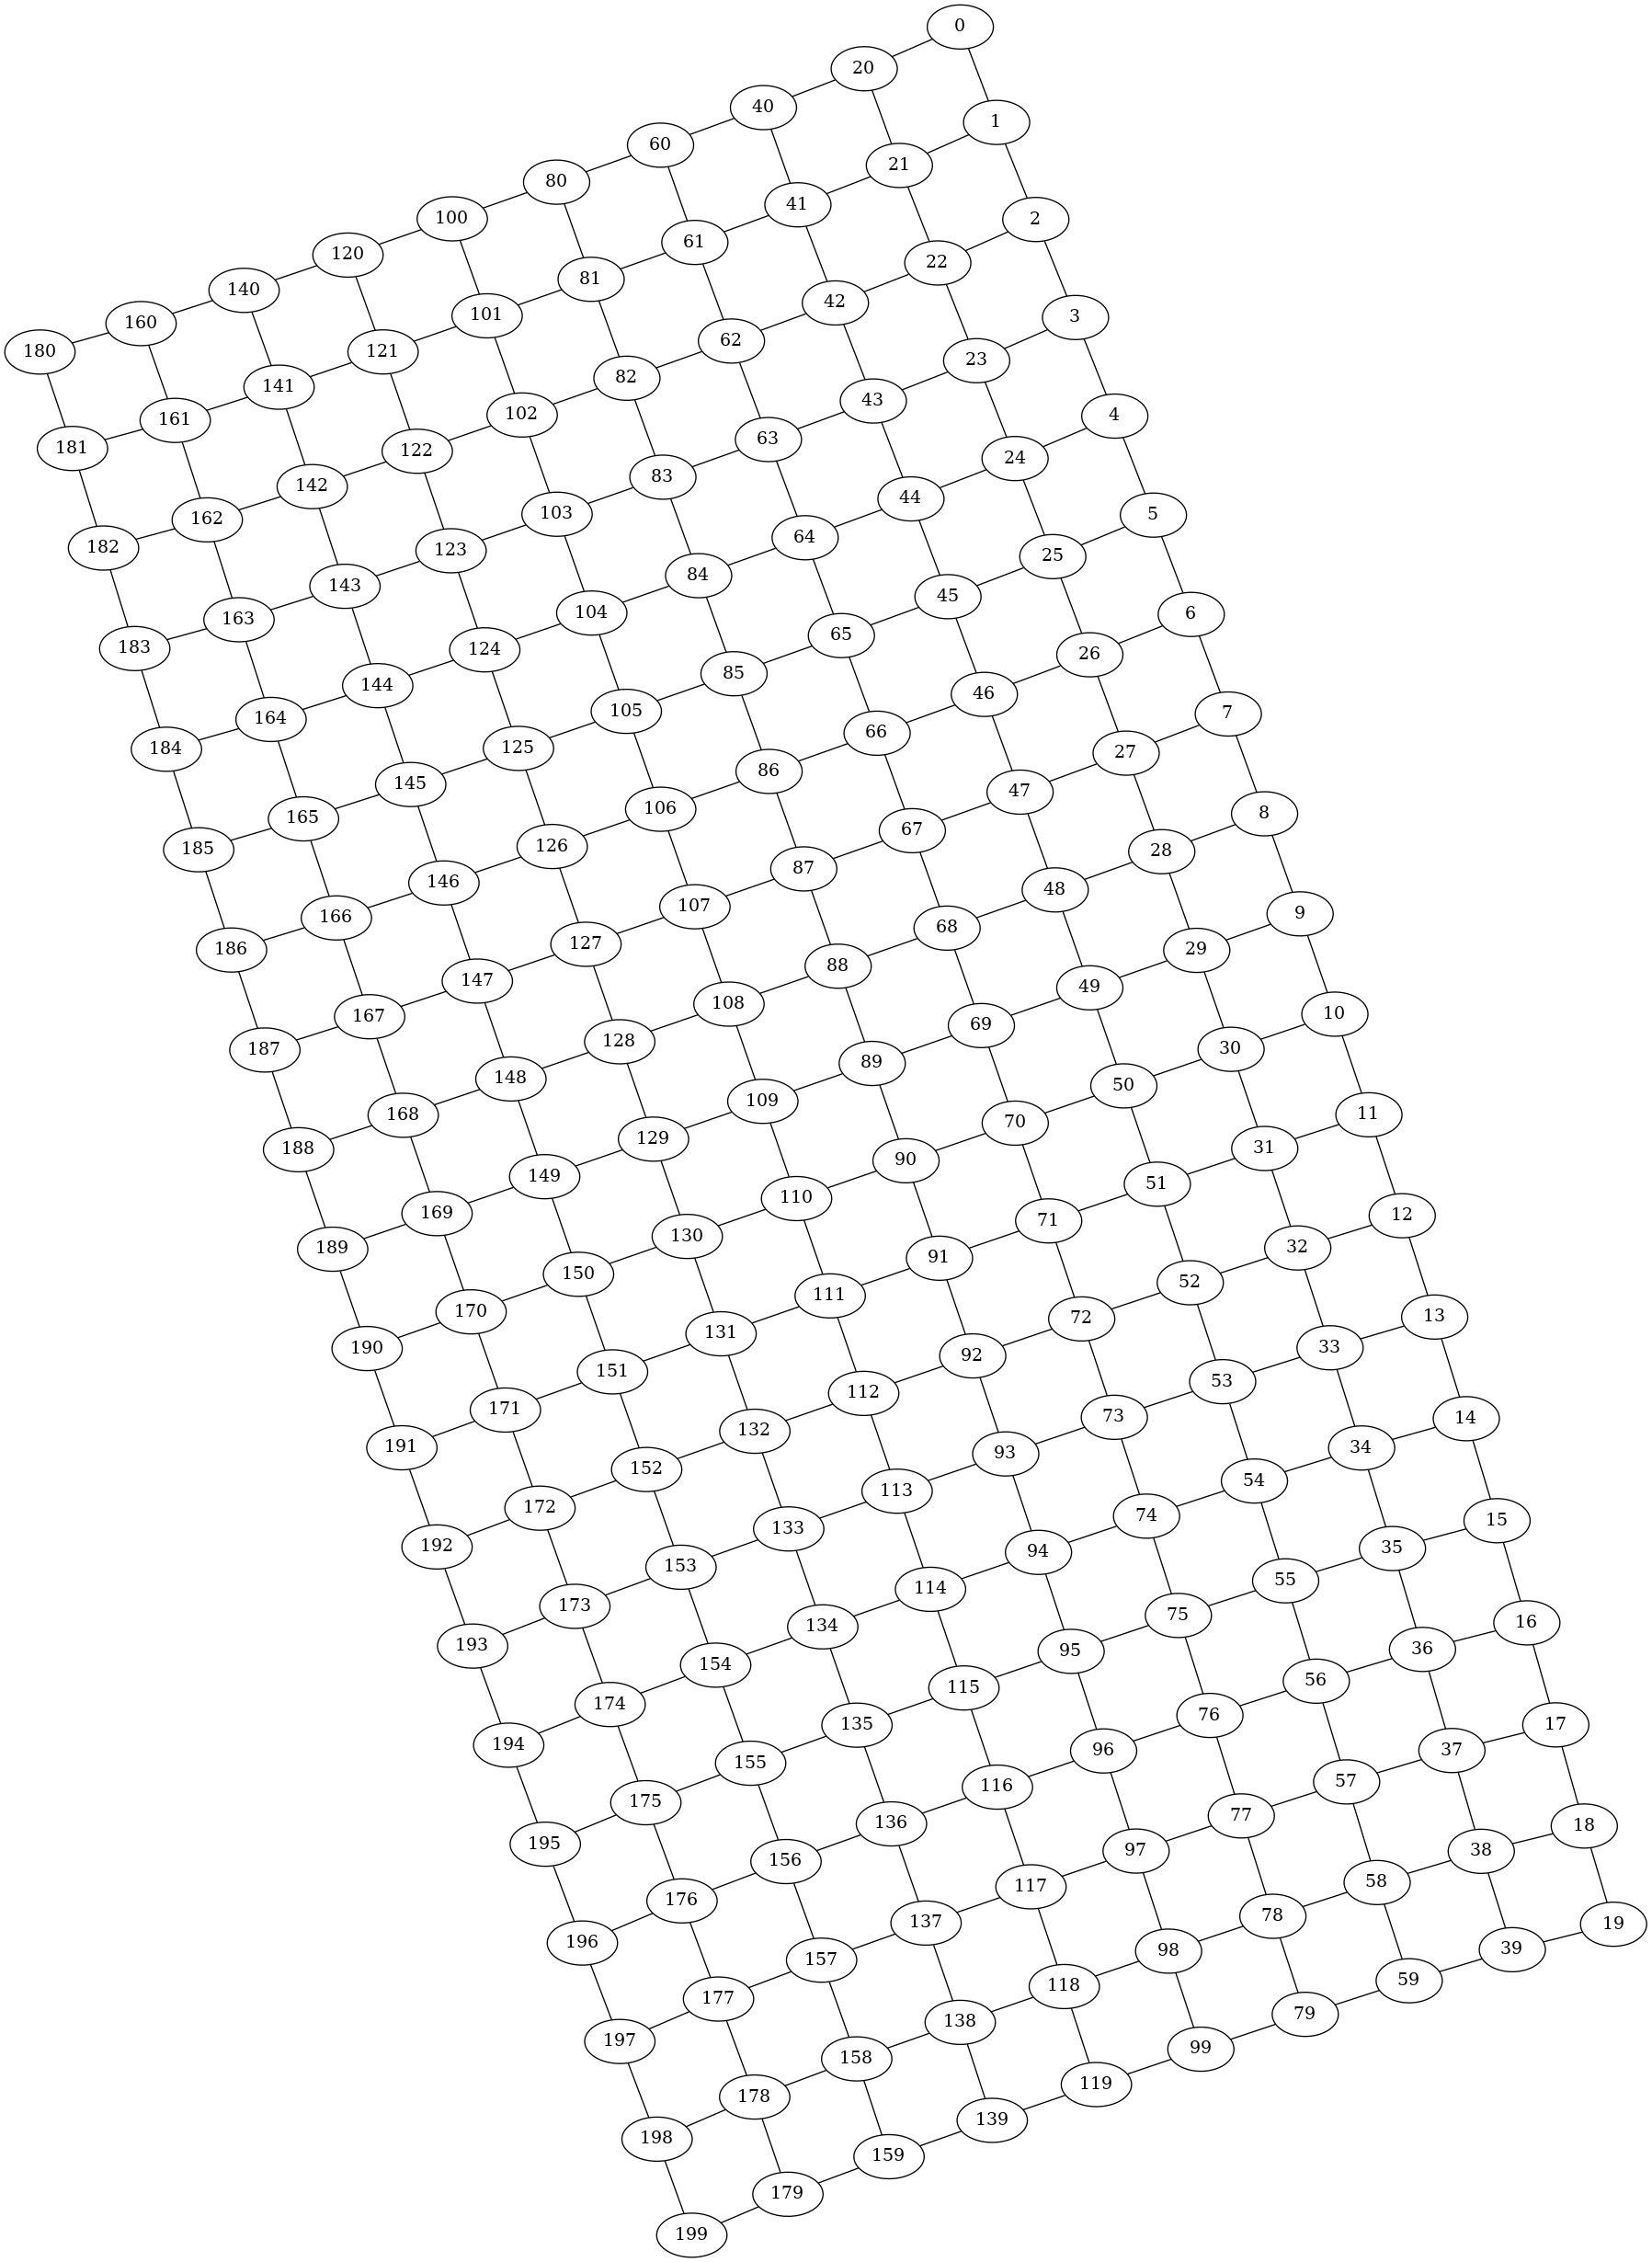
\includegraphics[width=0.4\linewidth]{004_team_1_agent_design/images/sc_network_grid.png}
%     \caption{Grid initialisation of 200 agents}
%     \label{fig:sc_network_grid}
% \end{figure}

%The network value of an agent can be initialised at the start of the game. For example, agents can be initialised in a grid structure (figure \ref{fig:sc_network_grid}) where most agents are connected to four other agents, aside from agents at the edges or corners that are only connected to three or two agents respectively.

% \begin{figure}[!h]
%     \centering
%     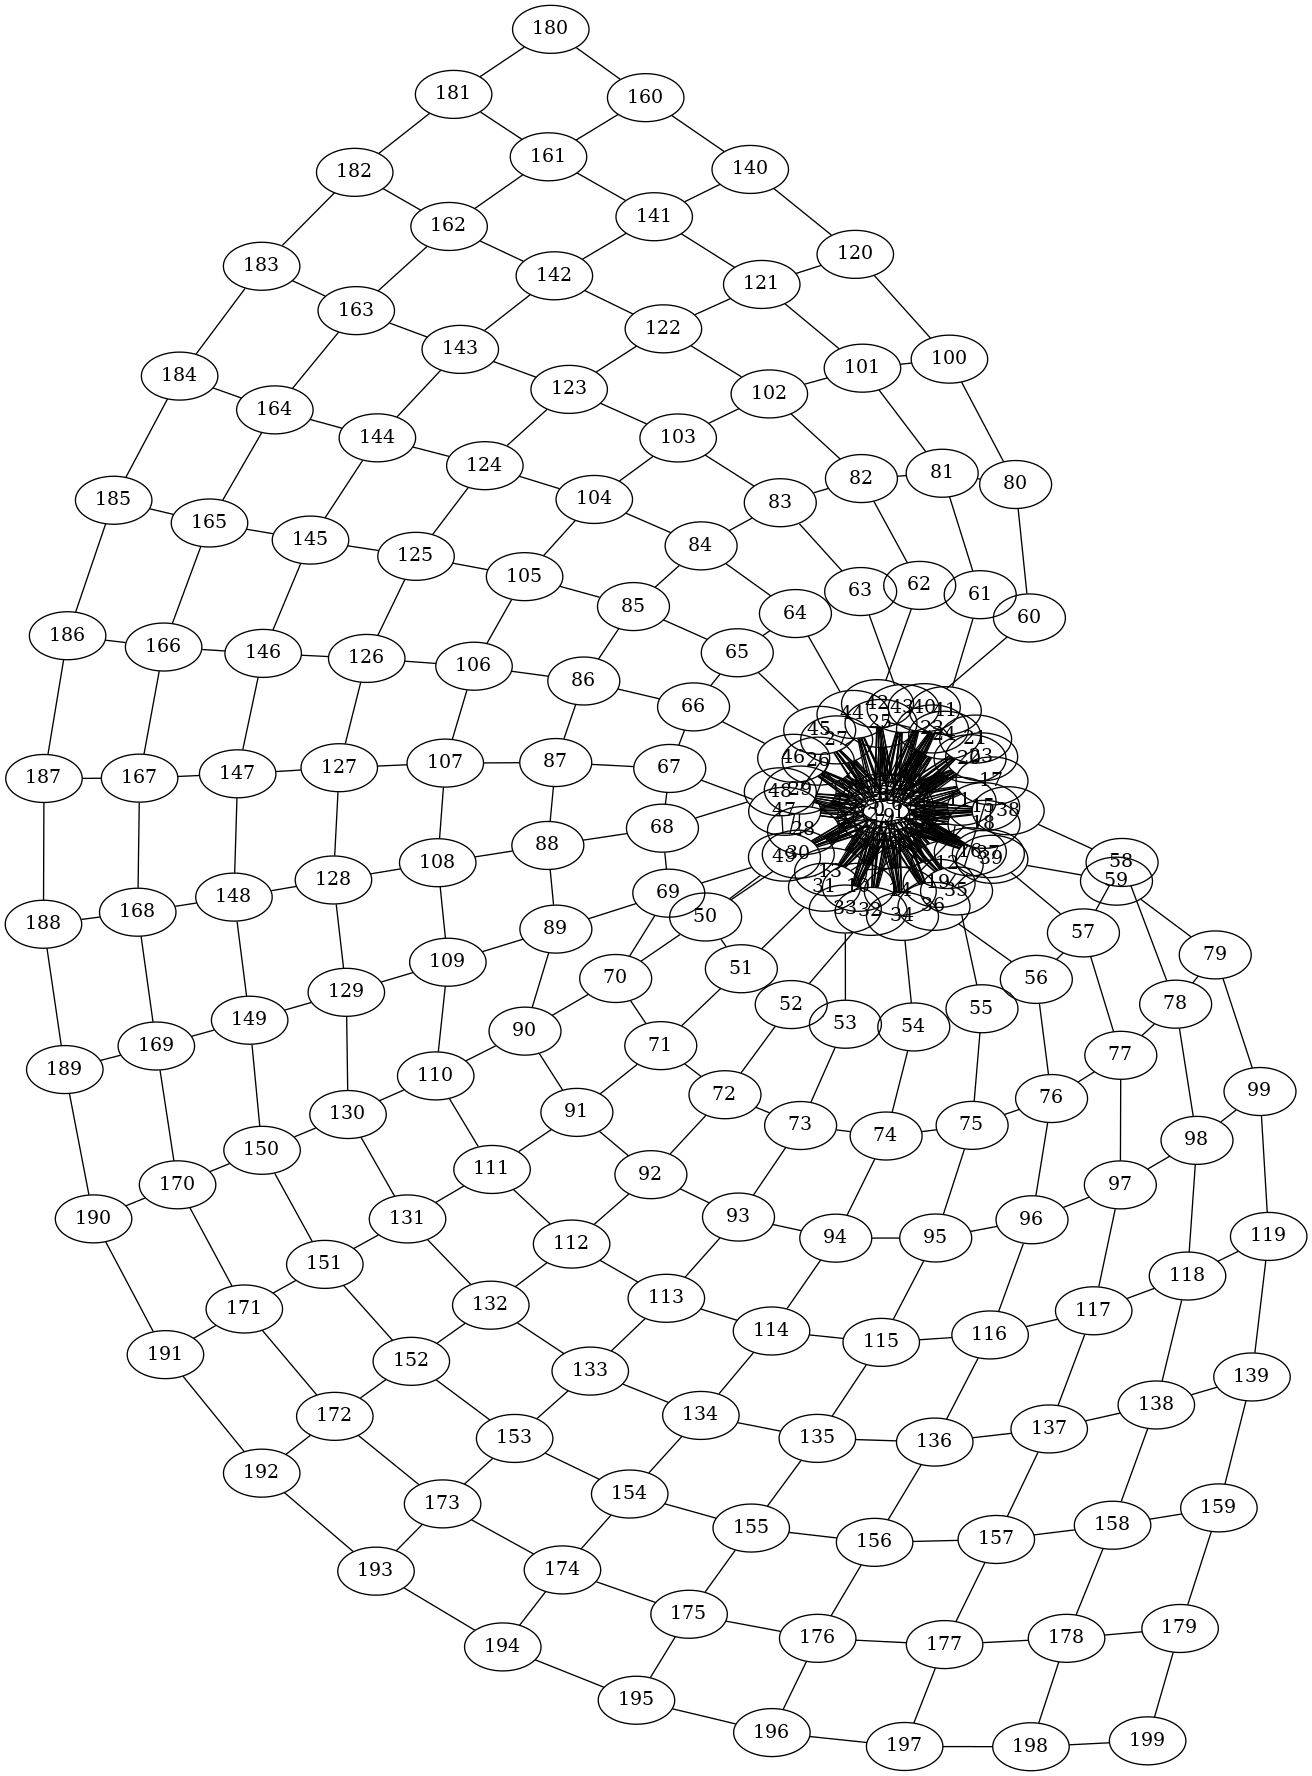
\includegraphics[width=0.4\linewidth]{004_team_1_agent_design/images/sc_network_clique.png}
%     \caption{'Clique' initialisation of 200 agents}
%     \label{fig:sc_network_clique}
% \end{figure}

\begin{figure}
\centering
\begin{minipage}{.5\textwidth}
  \centering
  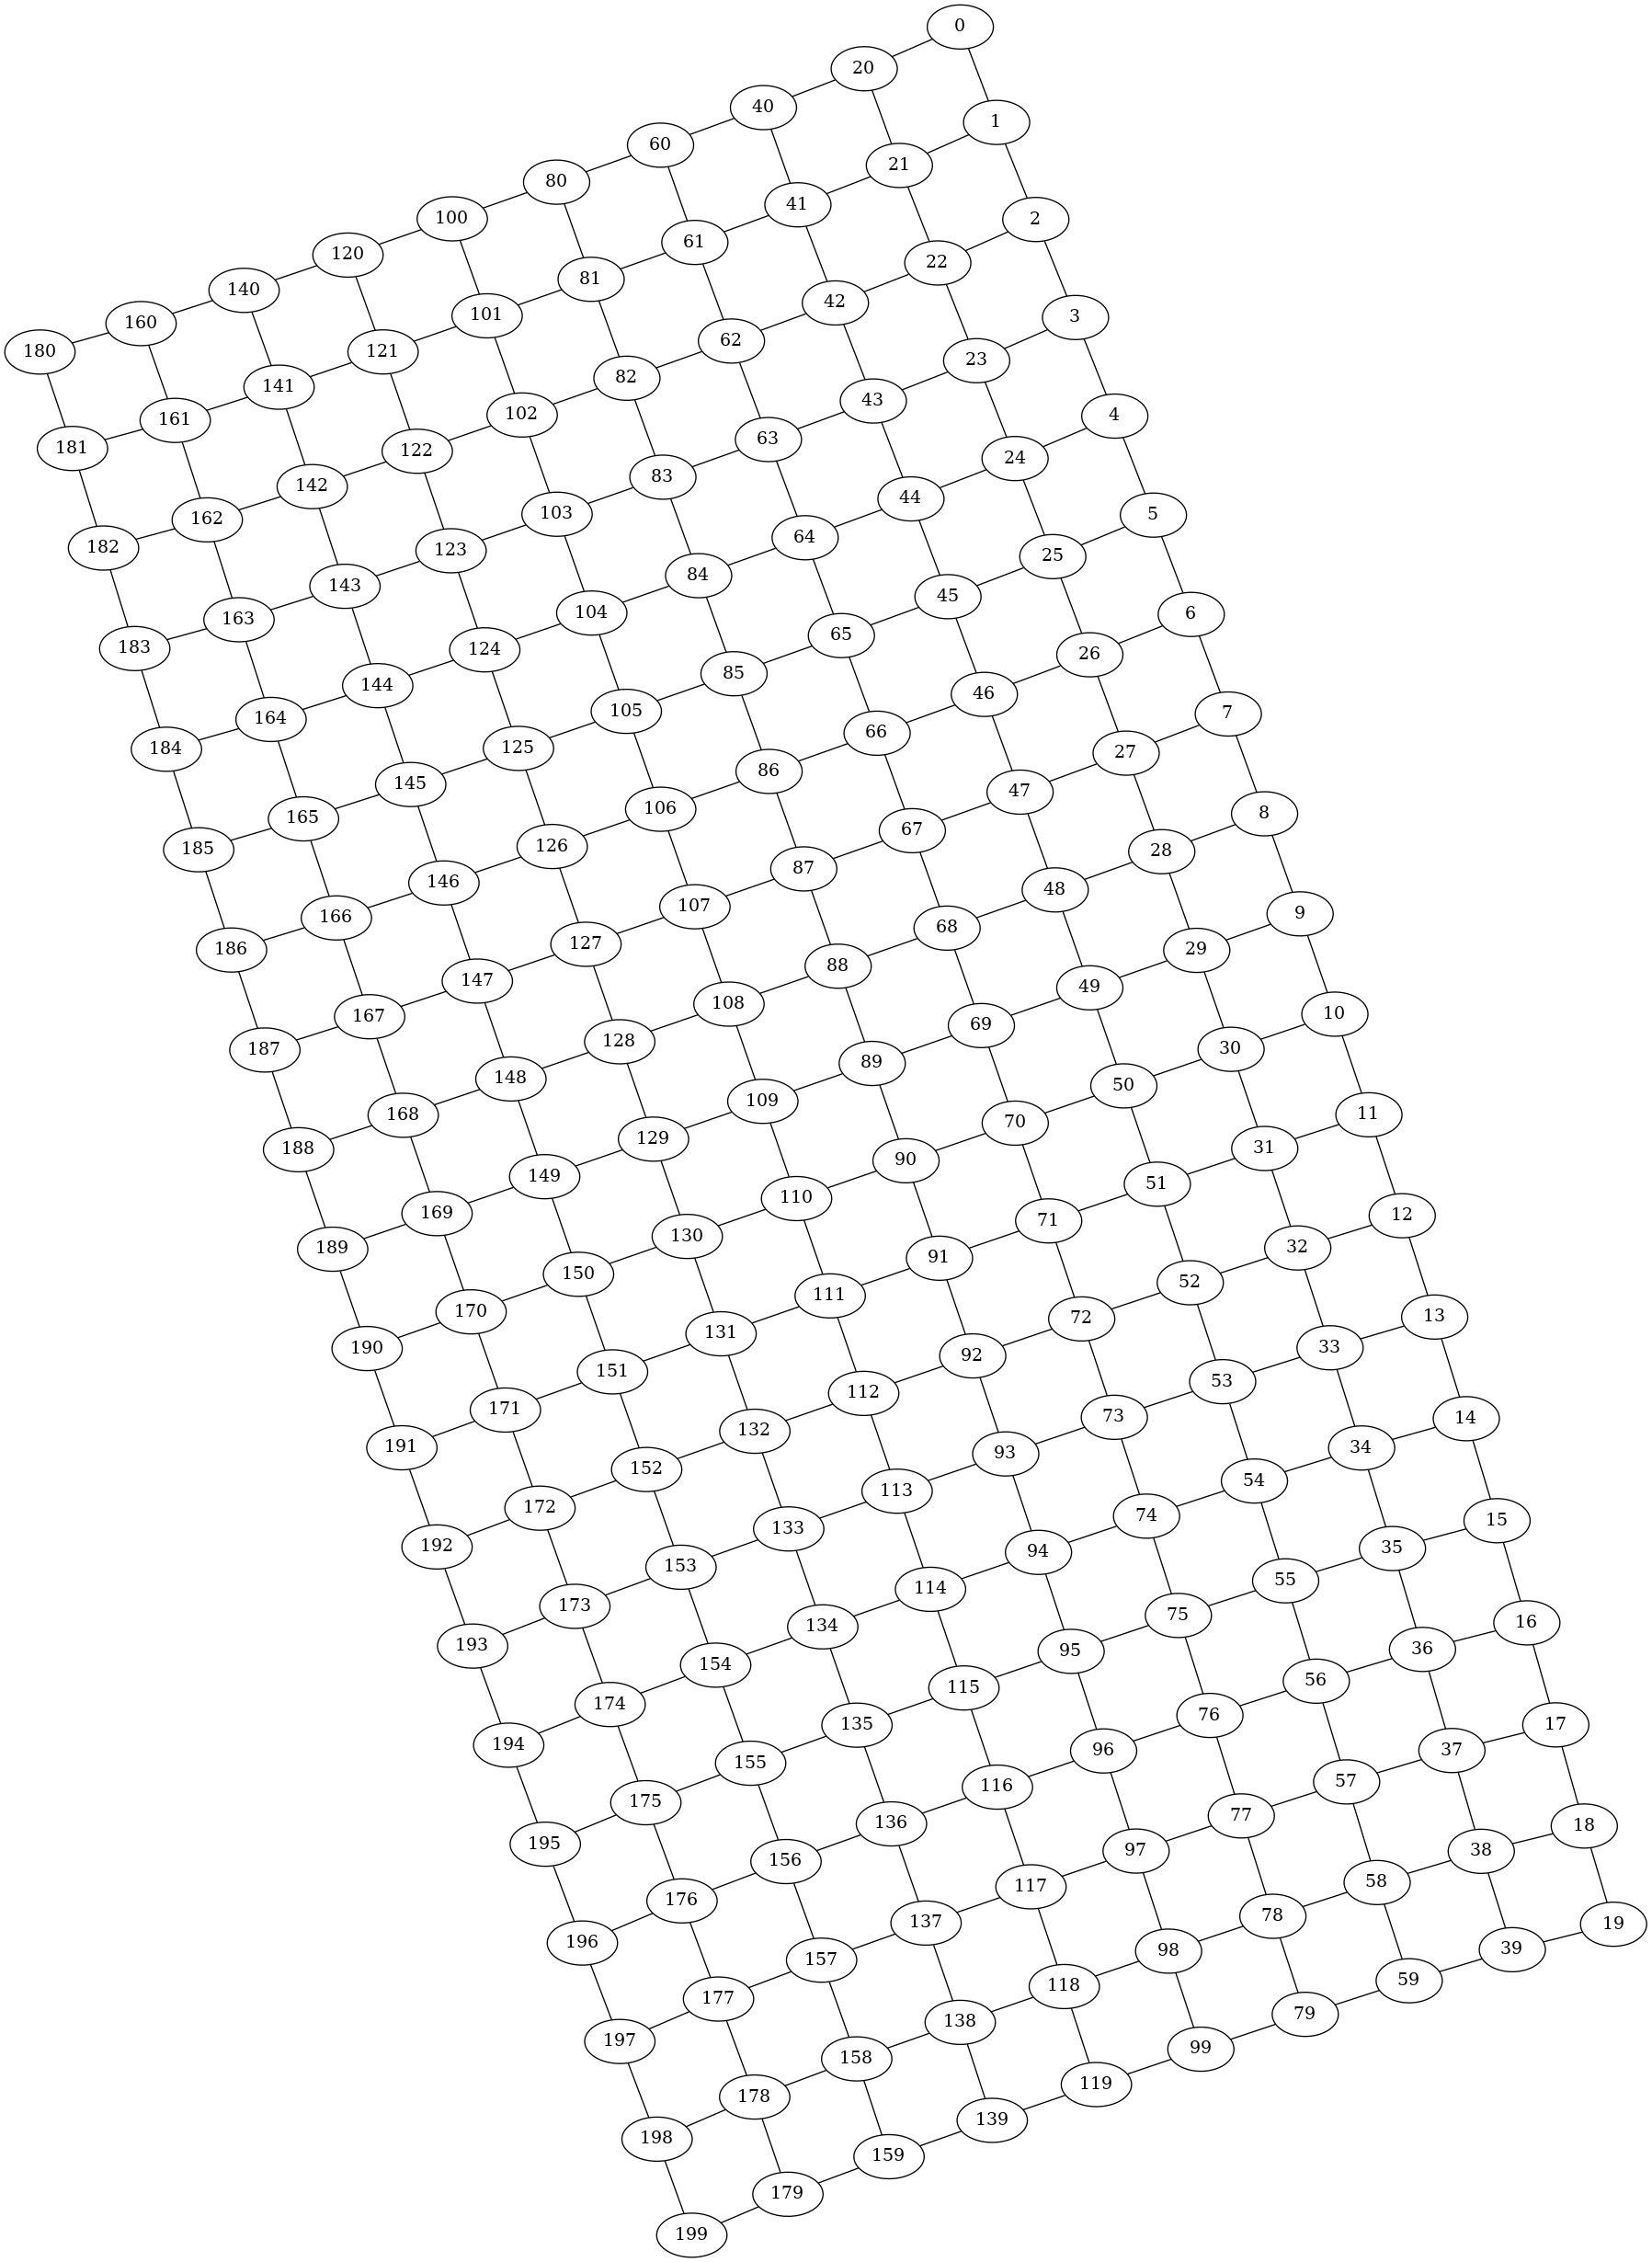
\includegraphics[width=.8\linewidth]{004_team_1_agent_design/images/sc_network_grid.png}
  \captionof{figure}{Grid initialisation of 200 agents}
  \label{fig:sc_network_grid}
\end{minipage}%
\begin{minipage}{.5\textwidth}
  \centering
  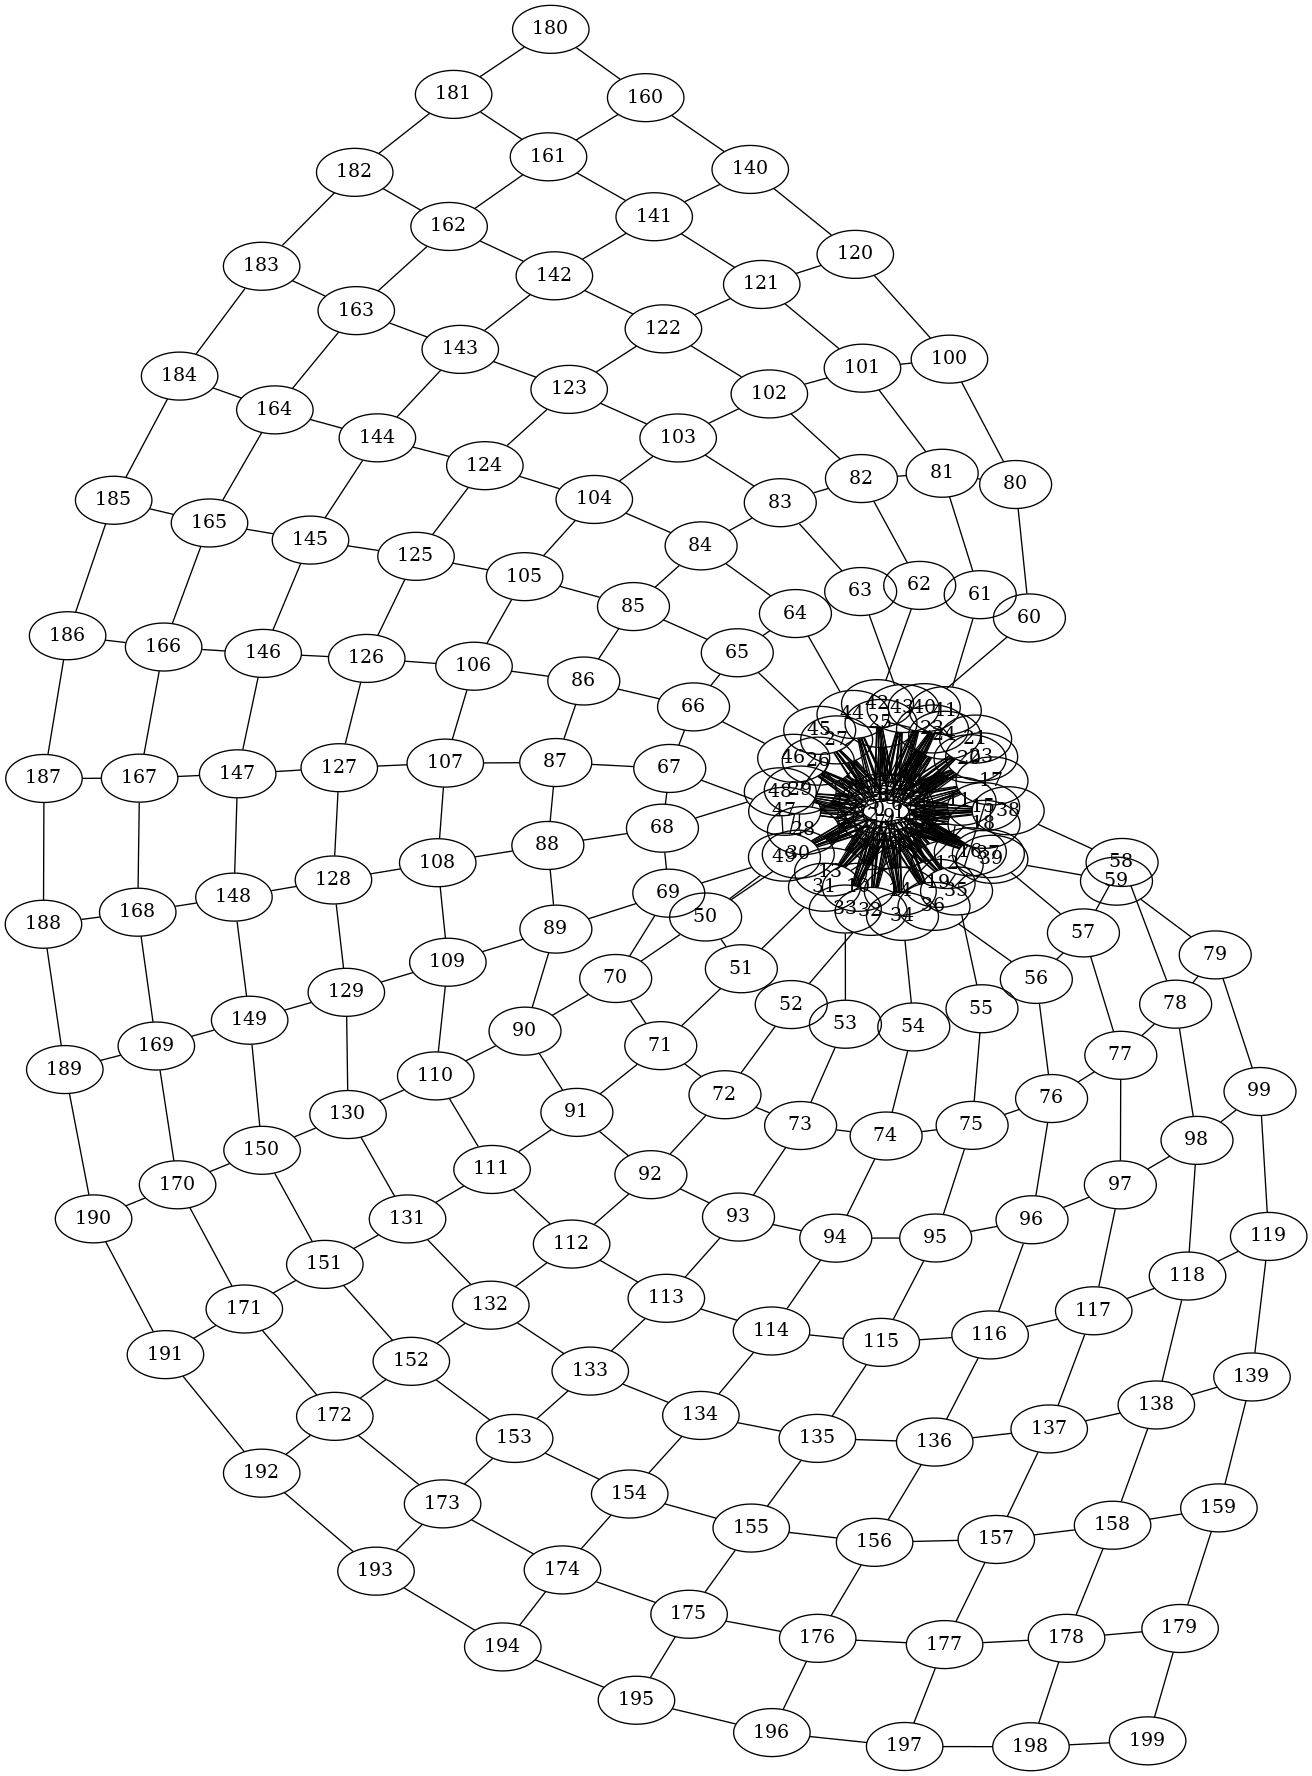
\includegraphics[width=.8\linewidth]{004_team_1_agent_design/images/sc_network_clique.png}
  \captionof{figure}{'Clique' initialisation of 200 agents}
  \label{fig:sc_network_clique}
\end{minipage}
\end{figure}

More complex initialisation patterns can also be explored. Figure~\ref{fig:sc_network_clique} shows a 'clique' initialisation pattern, where the first 10 agents are all connected to each other and 40 other agents. Consequently, those next 40 agents are each connected to the first 10 agents with a few connections to the rest of the grid, producing three tiers of agents with connections.

These network connections can change during the game itself, and are updated as follows:
\begin{enumerate}
    \item At the start of each fight round, agents gossip to their connections about the $N_A$ agents with the highest average Trustworthiness and Honor values - thereby praising them. The number of agents gossiped about in the message ($N_A$) is given by 
    \[
    N_A = P_A * (\#alive\ agents)
    \]
    where $P_A$ is the proportion of living agents admired, currently set to $0.1$. A message is sent to the agent's connections containing a list of the agents and indicating that they are being praised.
    \item The same happens for agents with the lowest average Trustworthiness and Honour values, with a proportion of alive agents disliked (set to $0.1$) being denounced.
    \item Upon receiving praise from an agent A about agent B, the agents network value of B increases, while the opposite is true if agent B was denounced. The network value of agent B changes based on the following formula:
    \[
    network_B += sign * perception_A * 0.1 * network_B
    \]
    
    Where $sign$ is $+1$ if the agent is praised and $-1$ if the agent is being denounced. $perception_A$ is the overall perception (average social capital value) of the sender. This means that if the sender has a negative social capital value then the effect of the senders message is actually reversed.
% TODO: Update these once we twweak the calculations in the game
\end{enumerate}

In the above update stages agents do not praise or denounce themselves, though an agent may directly tell another agent that they are praising or denouncing them through these messages.


\subsection{Trustworthiness}

In their 2007 paper Ostrom and Ahn give multiple examples of trustworthiness, but give no concise definition. One definition fitting the examples of Ostrom and Ahn is that given by Pitt in his 2021 book on Self-Organising Multi-Agent Systems: "Trustworthiness, as distinct from trust, and related to reputation, being a shared understanding of someone’s willingness to honour agreements and commitments"\cite{pitt}. In their paper, Ostrom and Ahn treat trustworthiness as a function of an individuals observable characteristics such as appearance, dress, gender, age and language. Moreover, they give examples of so called "one-shot" situations in which an individual has to decide on whether to trust another individual which they have never previously interacted with.\cite{ostrom-ahn}

Given that agents' interactions in the Escaping the Dark Pit(t) game are not one-shot, but repeated, handling trustworthiness as an inherent property of an agent's current observable characteristic is not ideal. Instead, as agents interact many times, it is more natural to use previous interactions to estimate future cooperativeness. Our agent therefore does not use observable characteristics to determine trustworthiness, as Ostrom and Ahn did. Instead, we define an agent's trustworthiness in the following way: "Trustworthiness is an agent's tendency to cooperate with and trust other agents as evidenced by their past actions."

Each agent updates the $Trustworthiness$ social capital value of other agents at the end of the round in the following way: The agent takes in the other agent's current state and passes it through its Q-functions. The Q-functions then give the potential social welfare of each of the agent's possible actions. Depending on their utility to the group, each action is placed on a scale from -1 to 1. Where the value of 1 is given to the most beneficial action and -1 is given to the least beneficial action. Actions which are neither the best nor the worst are assigned a value by interpolating between -1 and 1 based on the social welfare of the action. With every action assigned a cooperativeness value between -1 and 1, the agent now reads in the selected action of the other agent and links it to the cooperativeness score between -1 and 1. Finally, we multiply the cooperativeness score of the action by 0.1 and add this to the original trustworthiness score. Note that it is the decision on whether to attack, defend or cower which we use to update the trustworthiness score.

\subsection{Honour}
\label{subsection:honour}

The concept of honour should be well known by most, with one possible definition being that given by the Cambridge Dictionary: "to feel you must do something because it is morally right, even if you do not want to do it." Specifically, with the $Honour$ social capital value we seek to capture the feelings about the justness of an action. An example of a situation where such feelings could be encountered is when taking out the trash from one's shared apartment. Taking out the trash is a chore which few enjoy doing. As such, there is generally an unspoken agreement between tenants that they will share the burden of taking out the trash. If one tenant took out the trash the last time, the other tenant who did not take out the trash is likely to feel obligated to be the one who takes out the trash the next time. In this given situation, the feeling of honour ensured that burdens are fairly distributed. Similar feelings also come into play in situations where a person has been wronged. For example, if a tenant made themselves dinner and neglected cleaning the kitchen for several days, the other tenants may feel like it is just for them to have the same behaviour towards cleaning the kitchen. Based on these two examples of honour we can come up with the definition that $Honour$ is the running balance between favours and disfavours done for an agent and the favours and disfavours received from the same agent. 

To update the $Honour$ social capital value we use the difference between the cooperativeness score of the other agents' actions with the cooperativeness score of the agent's own action. This difference is then multiplied by 0.1 and added to the original $Honour$ value of the agent. An example is as follows: Let agent 1 have chosen to attack and agent 2 have cowered in a given round. At the end of the round, agent 2 will update the $Honour$ social capital value of agent 1 by first calculating a cooperativeness value for each of their actions in the same way as was done when updating trustworthiness. As cowering generally is an action which does not benefit the collective, agent 2's action will likely be given a cooperativeness value of -1. Inversely, attacking is generally a very cooperative action and will likely be linked to a cooperativeness value of 1. Agent 2's new $Honour$ social capital value for agent 1 will then be given by:
\begin{equation}
    Honour_{new} = Honour_{old} + 0.1*(1 - (-1)) = Honour_{old} + 0.2
\end{equation}

Note that as for all other social capital values, $Honour$ has a maximum value of 1 and minimum value of -1.

% \section{Social Bias}

% If the aim of the entire game from the point of view of each agent was to get as many agents as possible to escape the pit without regard for whether they themselves make it out, all agents would simply implement whatever the optimum strategy is to maximise total agent survival (although this strategy can be relatively difficult to find). However, since every agent also wants to ensure it is one of the surviving agents, the game becomes a  competition to ensure a place amongst this surviving group. This concept introduces the idea of punishing agents with bad social capital, resulting in agents attempting to see how much selfish behaviour they can get away with before the negative social consequences outweigh the potential gain. Thus in order to incorporate this logic into our agents decision making, it is important to not only maintain a score of social capital of other agents but also an estimation of what the collective group's opinion is of our agent. This value can be fed into our decision making to adjust the selfishness and cooperation of our agent if it finds that the group has a bias against it. 

% In order to measure the social bias against our agent at each round we try and estimate whether or not we are being punished. What constitutes a punishment can again be very difficult to define as this requires knowledge of what a good game position is, which in turn requires knowledge of the optimum strategy. To simplify this problem, our agent assumes that being made to fight is generally a bad thing as this can lead to loss of health, therefore, we need to try and keep track of whether or not our agent is made to fight more often than it should. The algorithm devised for this makes use of the survival likelihood scores mentioned earlier to find a set of agents in a similar position to our own agent and using the standard deviation of this score to adjust the threshold of similarity. Once the set of agents similar to our own has been found we can then find the fraction of this set of agents that were made to fight and also the boolean value of whether our agent is made to fight. What we are trying to measure using these two variables is whether there is a statistical difference in our fight frequency compared to what we would expect it to be. 
% An exponential weighted moving average is formed in order to accomplish this with the following algorithm showing how this average is updated at each round. 

% \begin{align*}
% \text{If agent is made to fight:} \\
% biasAverage \leftarrow (1-e)*biasAverage + e*(1-ratioMadeToFight) \\
% \text{Else} \\
% biasAverage \leftarrow (1-e)*biasAverage - e*(ratioMadeToFight)
% \end{align*}

\section{Selfishness}

Another core element of our agents is selfishness. With selfishness we mean a tendency to do actions which promote one's own utility rather than the utility of others. In our agents, selfishness is represented by the $selfishness$ variable, a float value between 0 and 1. A $selfishness$ value of 0 indicates that when choosing an action the agent only considers the benefit to the collective, while a $selfishness$ value of 1 indicates that the agent only considers an action's benefit to oneself. Any agent with a selfishness value between 0 and 1 will consider an action's benefit to both themselves and the collective. At the beginning of each game each agents' $selfishness$ value is initialised to a random value in the range $[0,1]$. 

%Weighting of how much agent prioritises its own performance over the performance of the group as a whole.

\subsection{Impact on Decision Making}

The selfishness value is used when agents decide on what fight action they want to take. For deciding on a fight action, each action passes their current state through their Q-functions. The Q-function then calculate the expected utility of an action for both the individual and the group as a whole. For each action, the agent then aggregates the two utility values into a single aggregated utility value using the following formula:

\begin{equation}
    Q_{action} = selfishness*Q_{self} + (1 - selfishness)*Q_{coop}
\end{equation}

In this formula $Q_{self}$ is the estimated utility value of an action to the agent itself and $Q_{coop}$ is the social welfare of the action. After aggregation, the agent then chooses the action which has the highest aggregated utility value. From the formula, it can quickly be deduced that any agent with a high degree of selfishness first and foremost will consider the estimated utility of an action to themselves rather than the utility for the group.

If the decision outputted through this process does not match the action our agent should take given the Ostrom Rule proposals voted on by the group, our agent must make a decision on whether to ignore these rules. To do this we take the expected reward of all three possible actions and scale the values such that the minimum reward is -1 and the maximum reward is 1. We than scale add $3*(1-selfishness)$ to the reward for the action proposed by the rule system. If this outputs a value greater than $1$ we go with the rule action, otherwise we go with the Q-action. This result of this system is that agents with higher selfishness are more likely to ignore the will of the group. 

\subsection{Updating Selfishness}

Similarly to social capital, the $selfishness$ value is updated at the end of each round. To update its own selfishness value, each agent starts by creating a slice containing the id of every other agent which currently has a better state than the agent itself. To determine if another agent has a better state than the agent itself, it calculates the geometric mean of the HP, stamina, total attack and total defense of the other agent and of itself. The agent with the higher geometric mean is then considered to have a better state. After having identified agents with a better state, the agent uses its social capital map to calculate the average trustworthiness of those agents. It then compares this average value to the trustworthiness value it has stored for itself. If the trustworthiness value of the other agents is higher than the agent's own trustworthiness value, the agent decreases its $selfishness$ value by 0.01. Inversely, if the other agents have a lower trustworthiness, the agent increases its selfishness by 0.01. Finally, if no other agents currently have a better state, then the agent does not modify its $selfishness$ value.

With this updating method we have assumed that an agent's social capital $trustworthiness$ value is negatively correlated with their selfishness value, which should hold true given how trustworthiness is updated. In essence we then use the $trustworthiness$ value of an agent to estimate their selfishness. This way, an agent indirectly checks whether the agents which are performing better than it have a higher internal $selfishness$ value than them. The agent then adjusts their own $selfishness$ in the way which would make their behaviour emulate that of high-performing agents. It is hoped that through the sanctions imposed on non-cooperative agents, highly selfish agents will perform poorly, and thus agents are incentivised to reduce their selfishness over the course of the game. However, in initial tests we actually saw the average selfishness increase over the course of the game. Though more investigation is necessary to come to a clear conclusion, a potential explanation for these results is that the sanctions currently available for punishing selfish behaviour are too weak. 

\section{Forgiving and Forgetting}

As was shown in the previous section on selfishness, the agents' behaviours are dynamic and over the course of the game an agent which started out as very selfish might over time become very selfless or vice versa. With dynamic agent behaviours, recent actions are a better indicator of future actions than actions which an agent took far in the past. As such, it is beneficial for recent actions to hold greater importance when calculating social capital values than old actions. To achieve this goal we added a mechanism to "forget" an agent's previous action. The mechanism works by decaying the stored social capital values for all of the agents. Specifically, the algorithm used was the following:

\begin{verbatim}
    for each indicator in socialCapital:
        if (indicator < 0)
            indicator = 0.90*indicator
        else
            indicator = 0.95*indicator
\end{verbatim}

The exception to this formula for decaying social capital values was the $Institutions$ value. As has previously been discussed, technical limitations make it hard to compute updates for the $Institutions$ value. With little new information on an agents tendency to adhere to the norms of the institutions, it was decided to be wise not to forget past actions.

As can be seen, negative social capital values (or indicators) decay faster than positive social capital values. The reasoning for this is that we seek to make agents cooperate. If agents hold negative social capital with each other this can cause non-cooperative actions to be taken and therefore more negative social capital to be produced. By quickly decaying negative social capital we seek to eliminate such negative social capital loops and make it easier for agents to give others second chances. Moreover, if it was instead positive social capital which decayed faster, agents would be pushed towards trusting other agents less, achieving the opposite of our goal. We also believe this mimics human behaviour. For example, it is very common that individuals can have heated fights one day and despise the other person, only to forgive them the next day. However, the inverse seldom happens. If a person strongly likes a person one day, it is unlikely that they will stop liking that person the next day without any interaction between the two.

\section{Sanctions}
Since our agent design is based on a society using Ostrom-style rules it is important to have a mechanism to punish agents that aren't following these rules and act against the interests of the group. In the current game, there are few ways in which agents can directly influence the state of another agent, with the one exception being trade. As such, we use the trading mechanism as a way of imposing punishment.

\subsection{Exclusion from Trading}

Should an agent have a spare weapon in their inventory, an agent would decide to gift the item to another agent without expecting any item in return. This is performed by first selecting a random subset of 10 agents (or less if less than 10 other agents are alive at this point). The item is then offered to the agent of the 10 with the highest positive social capital.

The purpose of choosing a random subset of agents helps to spread out trades amongst agents and avoid many agents offering trades to just a select few agents with the highest social capital. An agent will skip making a trade to an agent if that agent already has a pending trade with itself, since a trade requires multiple rounds to be accepted.

Crucially, an agent will not make any trades to agents with a negative social capital even if there are no other agents left. This imposes a form of punishment on agents that do not follow the rules and further encourages agents to act in the interests of the group.

\section{Elections}

\subsection{Fight Proposal Creation}

In order to engage in the proposal system, our agent requires a mechanism to build proposals to suggest to the collective that align with what it believes is an optimum strategy to maximise the total agent survival rate. In order to do this, the possible state space in which any agent can exist is split into discrete ranges using four variables. These variables are the agents health, stamina, attack and defense. The health and stamina variables are each split into three ranges corresponding to the three possible ranges present in a hidden agent state (Low, Medium and High), and the attack and defense ranges are split into the either greater than the average attack or defense or less than the average. This gives in total 36 different agent states that can be passed to the Q-Learning functions to output the optimum fight decision to maximise group survival for a given agent state. 
We can then compose a rule using conditions on these discrete ranges and propose the action that these conditions should result in. The result of this is a proposal with 36 rules which can be submitted to the group.

\subsection{Fight Proposal Voting}

When deciding on whether or not our agent should be in favour of a proposal, we first try and measure the accuracy of a proposal as compared to the strategy given by our Q-Function. This is a measure of agreement with the proposal. We do this by finding the action the proposal would result in for each agent using the state knowledge we have and the action our system suggests, creating an overall percentage accuracy for all agents. In order to prevent $O(n^2)$ complexity, we compute the accuracy on a sample of the population of a constant size, in this case 20.  We then check if this value is above a given threshold and if so, vote positively. Since we have to vote on proposals as they come in and we don't know what future proposals may look like before voting on the current one, we modify our threshold system to account for this. For each proposal that we receive, if we haven't already voted positively on a proposal this game round, we slightly decrease the required threshold. If we don't vote positively on any proposals in a given game round, the starting threshold is slightly decreased. If we vote on the first proposal received, the threshold is slightly increased. The voting threshold is set to the current starting threshold at the beginning of each game round.

\subsection{Leader Election}

Our original strategy made use of a leader that had absolute power over fight decisions as a mechanism to sanction agents that had bad social capital. This resulted in a system where being the leader was often an undesirable position as it required punishing many other agents, resulting in bad social capital for that agent. However, since the game design was changed such that agents can always defect from the leaders decisions this system was entirely changed as the leader can no longer be used as a sanctioning mechanism. In this new system, leadership elections are greatly simplified and are now only dependent on the social capital of the agent giving a proposal, the length of the term and the overthrow threshold. The social capital score is shifted to lie between 0 and 1 (such that the greatest social capital is 1) before being squared. We then vote for the leader if we generate a random number less than this score.

\section {Leadership}

\subsection{Fight Resolution}

When our agent is the current leader we always have $fightDecisionPower$ which means we can tell other agents what fight decision they should make (although they can ignore this). In order to decide what agent should do what, we try to allow agents with higher social capital a greater chance of implementing the action that our selfish Q-function suggests they should make and for agents with lower social capital we suggest they take the action in the interest of the group. To accomplish this, we find the percentile position of each agent by sorting their mean social capital scores and then take the percentile (between 0 and 1) of this position. This percentile is then raised to the 8th power to give each agent a score. If we generate a random number between 0 and 1 less than this score the agent is told to make the selfish action otherwise it is told to take the cooperative action. The 8th power is chosen as it results in roughly $10\%$ of the agents being permitted to take the selfish action which we found to be an acceptable value. The fraction of agents permitted to act selfishly on average for a power of $n$ is given with the following equation.

\begin{align*}
\int^1_0 x^n dx = \frac{1}{n+1} \\
\frac{1}{8+1} \approx 0.1
\end{align*}

\subsection{Loot Allocation}

Since our learning based approach isn't trained on loot allocations we are unable to make use of any kind of reward function to decide on what loot each agent should receive. Our solution therefore simply tries to make the state of all agents as similar as possible as there is no real benefit to having a large spread in agent states. The only exception to this is that it is bad to give agents both a good weapon and good shields as they can only use one at a time. This exception leads to some amount of specialisation being good for the overall system depending on how many agents should be defending in each round. Our strategy gives each agent a score for each type of loot based on these factors. For example, the lower an agent's health, the higher their health potion deserving score is. We also increase these scores in line with social capital. Once these scores have been calculated, the cumulative distributions are found for all agents and a random number is chosen for each loot allocation within the range of this cumulative distribution. Using a binary search of the distribution the loot is allocated to the chosen agent. By adding this small amount of randomness instead of a purely logical solution we found a small increase in levels survived during early testing. This may be due to unforeseen bad edge cases in the overall strategy being averaged out.


\section{Q-learning}
The agents have two "optimal" strategies, cooperative and selfish, that helps dictate their next decision. The social capital framework controls how decisions are made on top of these strategies. Q-learning \cite{qlearn} is a technique used to measure the "best" action to take given the current state of each agent. This is being used to help determine the next fight action, which includes "attack", "cower" and "defend". 

\subsection{Variables}
We learn a model that can map the agent state to a particular reward or Q-value for the next action they can take. The following variables define what counts as part of the current agent state that this model takes in.
\begin{equation}
    State = \{HP, Stamina, TotalAttack, TotalDefense, MonsterHealth, MonsterAttack, 1/HP \}
\end{equation}

These variables are continuous for the agent's perception of itself. These were chosen as they were deemed the most important variables that would impact their next decision. 

All agents have two optimal strategies that help decide their next action.
\begin{itemize}
    \item \textbf{Cooperative strategy} - acting with the common good in mind and the survival of the collective
    \item \textbf{Selfish strategy} - optimises for the survival of just that agent
\end{itemize}
The cooperative strategy should assign the highest reward to the action that leads to the most utility for the collective and all agents living the longest on average. The selfish strategy assigns the most reward to the action that leads to that agent living the longest.

\subsection{Learning and reward function}
Each state must be assigned a reward that we want to learn to predict. For the cooperative strategy, the reward is the mean remaining number of levels that the remaining agents in that game live for after that action was taken. This is a measure of how that action actually helped the collective. For the selfish strategy, the reward is the remaining number of levels that that agent survived for in that game. These measurements can only be calculated at the end of a game. The training data is made out of a collection of decisions made for each action together with the associated collective and selfish reward.

There are several methods that could be used for Q-learning. A common method is to store the reward for each state in a table, although there are a very large number of combinations of possible state variables even if they were discretised to a smaller set of values like \{low health, medium health, high health\}. Therefore, we use linear regression instead, which maps the state to a reward. These functions are parameterised by a set of eight weights each as shown in equation~\ref{qregress}, and each function predicts the reward for one type of action. A strategy is made up of these three linear regressors for each action. There are two strategies that are learned, so six functions are set up. 

\begin{equation}\label{qregress}
\begin{aligned}
Q_{reward} = w_0 + w_1 * HP + w_2 * Stamina + w_3 * TotalAttack + \\
w_4 * TotalDefense + w_5 * MonsterHealth + w_6 * MonsterAttack + w_7 * 1 / HP
\end{aligned}
\end{equation}

\subsection{Training}
These weights are initialised randomly. They dictate the Q-values and the decisions made by the agents. Several games are run using this strategy and each agent decision is stored together with the state. Once each game ends, the cooperative and selfish rewards can be calculated and are added to the log. This data forms a training set and a least squares problem $State * W = Reward$. The $W$ can be calculated and forms the new weights for the agent. These steps are repeated using the new strategy with the new weights, so that the next set of weights can be calculated. Another approach that was tested was to update the weights according to a gradient descent function to learn the function approximation \citep{qlearnatari}. The update is in the direction of the gradient and weighted by the error between the actual reward and Q-function reward. Usually, the discounted future reward for the next state would also be taken into account to determine how the action impacts future performance, but rewards are calculated over an entire game in this setting, so the reward of that agent remains the same throughout the game.

Using a fixed greedy strategy that always takes the action with maximum reward throughout training may result in it collapsing to doing the same optimal strategy all the time and not trying different actions that actually may result in better situations in the future. Therefore, an exploration parameter was added, which sets the probability for the agent to diverge from the strategy and choose a random action instead. This allows for a bigger portion of the state space to be explored and is known as an epsilon-greedy strategy.

After several iterations of this training, the final set of weights for the cooperative and selfish strategies are frozen and used at test time for the actual games. The game is dynamic and many parameters can change. It wouldn't make sense to learn a set of parameters for each game configuration, so the adaptation to the current setting is done using the other parts of this agents including selfishness. These trained strategies serve as a pre-trained ideology of collective and selfishness for the agents that influence how they act in the current scenario.

\subsection{Q-values}
The training ended up being very unstable and not showing huge improvements in performance. The reward signals for cooperative and selfish strategies were very similar as agents tended to die together near the end. Therefore, it was very difficult to distinguish what action had been selfish or cooperative, since there was no way to see if one agent had profited from that action.

We adapted our approach by manually setting the weights of the Q-functions with our preconceptions of what would be a selfish or cooperative action and what got the agents to survive for the longest. For example, if the agent has high stamina, the cooperative action would be to attack. This reflects the idea that agents have a preconception of morality and the adaptation to the current game is done using social capital and the other parts of the agent.

Other variables could also be explored in the future. The current state only takes into account the variables of the agents rather than of the state of all agents at that time. For example, the health percentile out of all agents or standard deviation of attack at a certain point would give it an idea of the collective state of the game. This could help it learn a better q-function and stabilise training. The game could also have had mechanisms for agents to die earlier somehow or some way to measure if an agent was punished or rewarded for their actions other than the number of levels they live for. This would have served as a better reward signal for training the Q-functions.

\section{Visualising Social Capital}

To observe the relationship between social capital and other elements of the game, a method of visualising how social capital changes throughout the game was developed. In past work by Petruzzi, Pitt, and Busquets \cite{electronic_social_capital}, a graph data structure was used to store the $Networks$ social capital data between multiple agents. A visualisation of such a graph changing during a game would be useful in allowing further experiments exploring how different parameters has an effect on social capital, or how social capital in turn has an effect on the behaviour or performance of the agent. 

Although our implementation does not use a graph structure to store social capital during the game, a directed graph was generated at the end of each level. Each of these graphs were then converted to a visual image and multiple images representing different levels of the game were then combined into a video. Each still image in the video (Figure \ref{fig:sc_visual_img}) contains a directed graph where each edge represents an agent having a social capital value of above 0.5 in the eyes of another agent. The yellow vertex represents the leader in the current round, while the red vertices represents dead agents. The border around each vertex indicates the remaining health of the agent and varies from green (high health) to red (low health). A more interactive example can be found in the Appendix, \ref{ani:sc_visual_vid}.

\begin{figure}[!h]
    \centering
    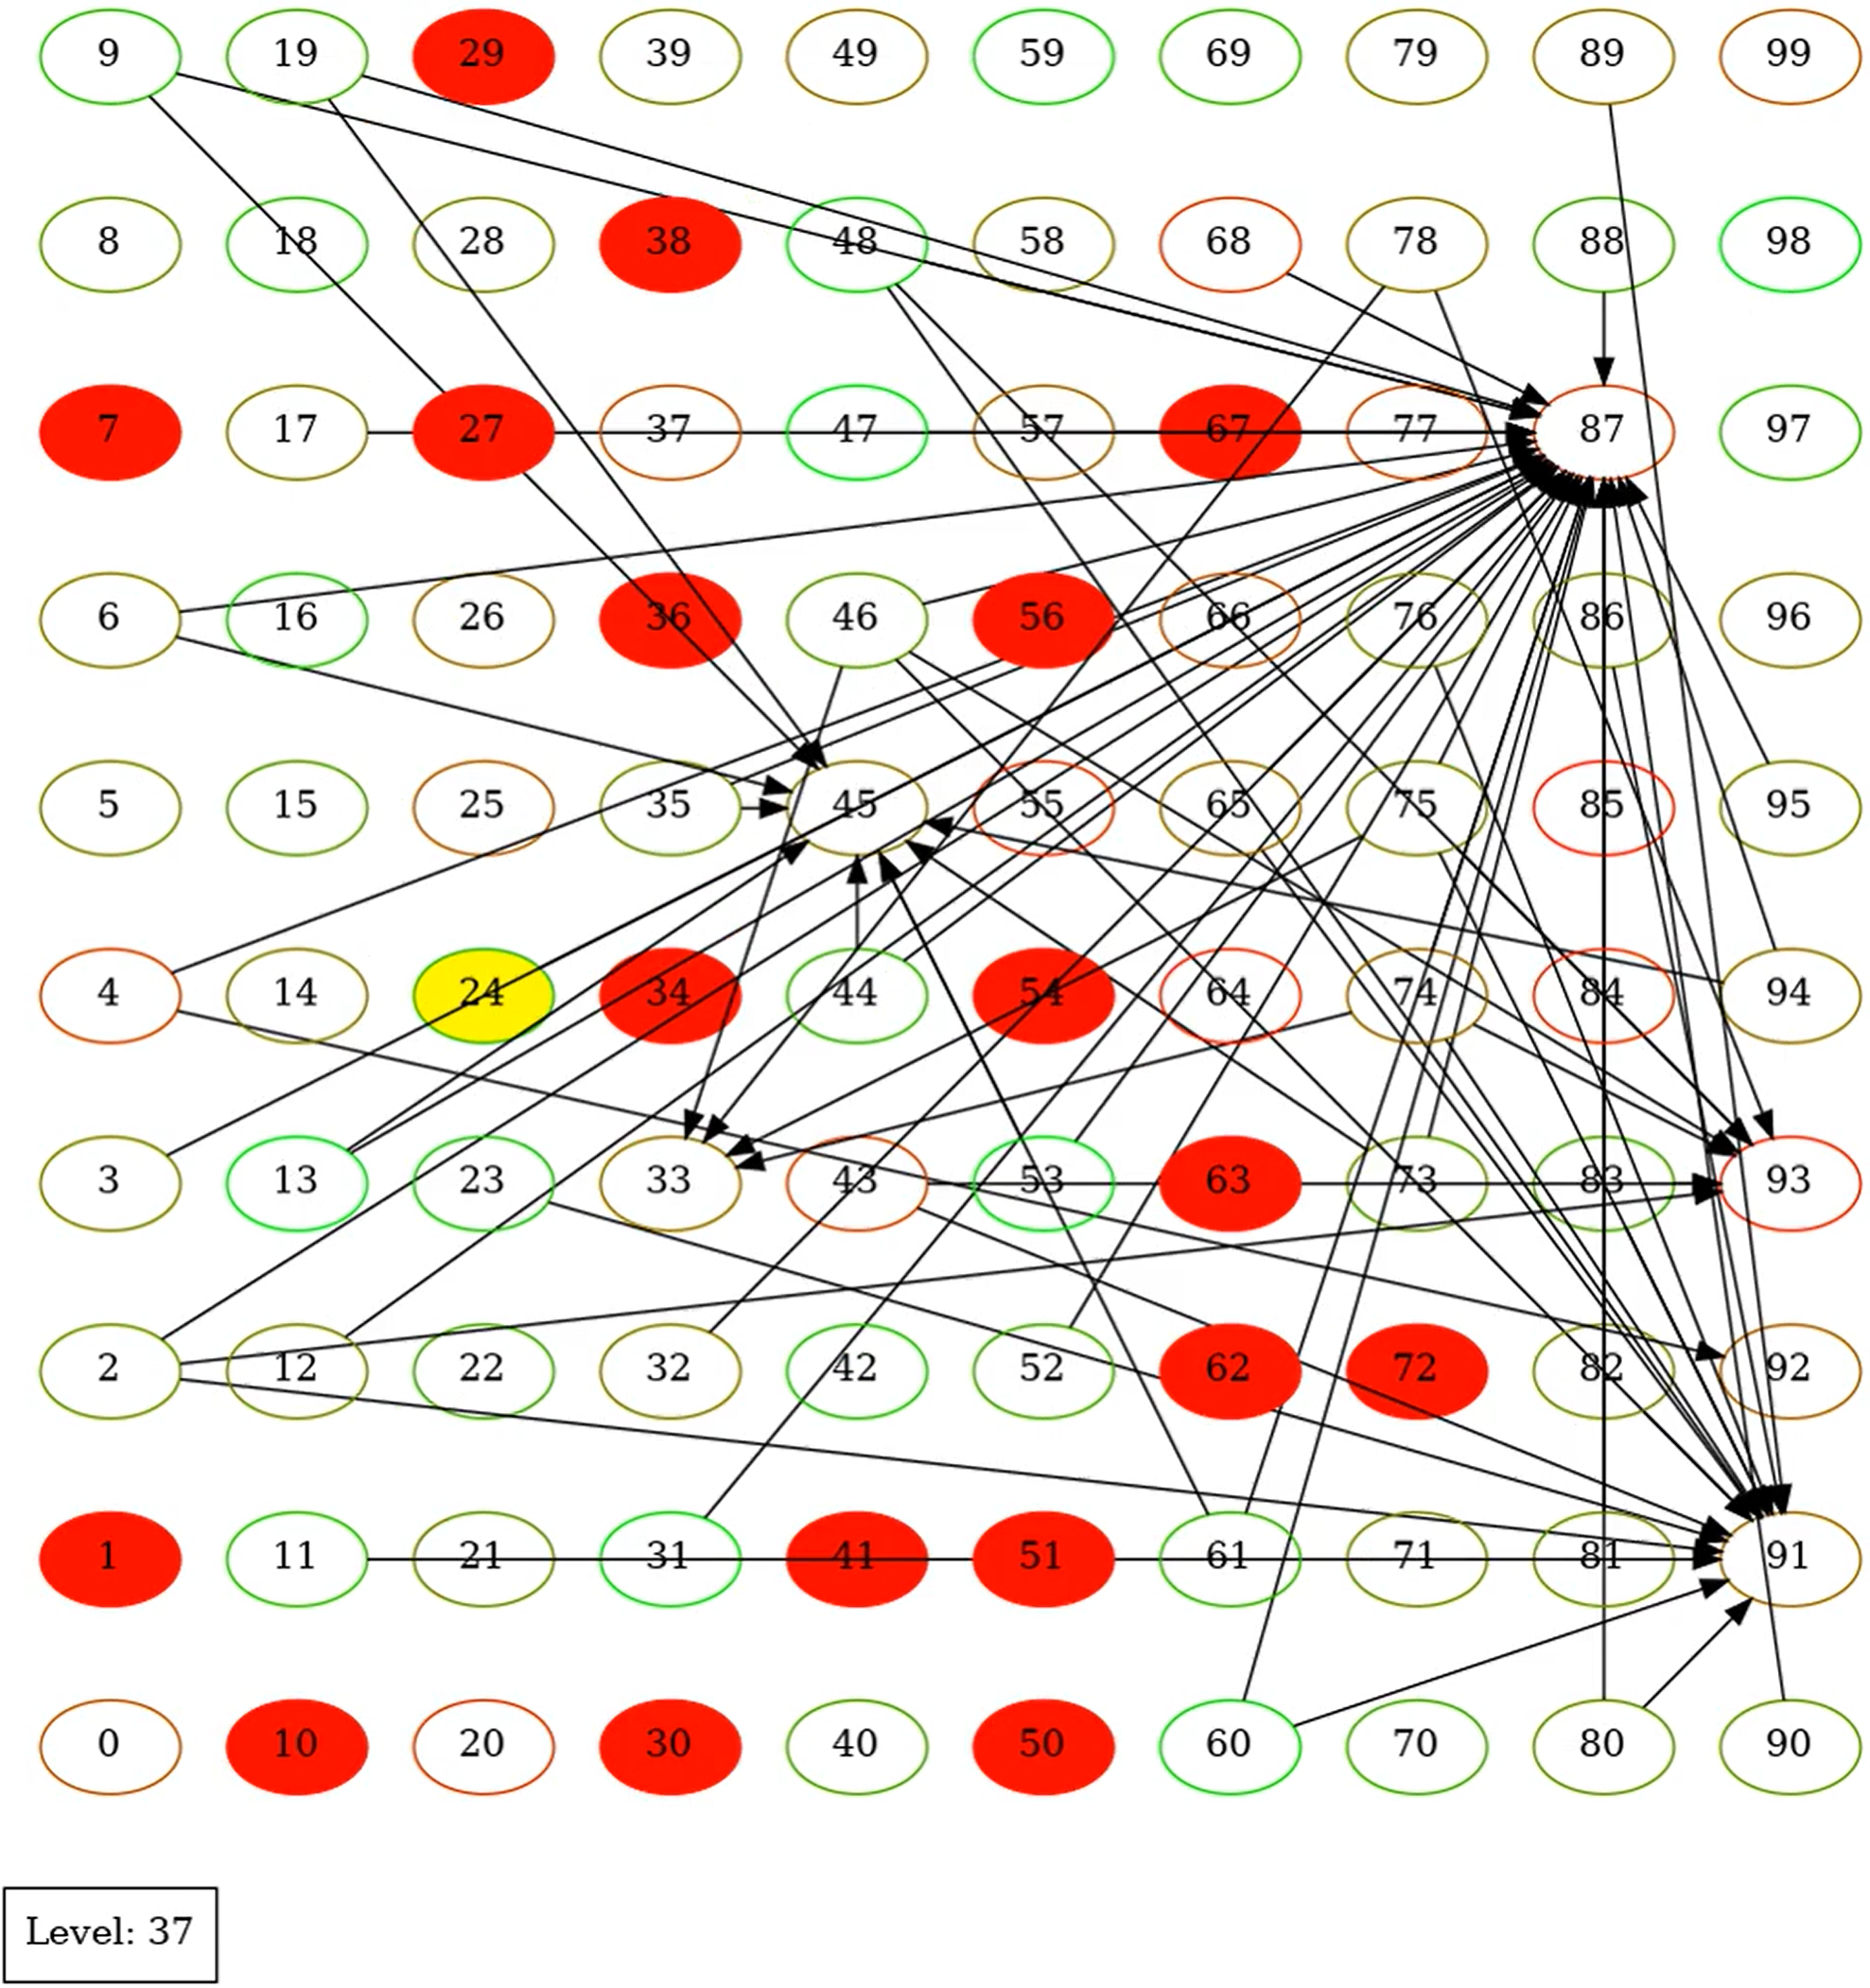
\includegraphics[width=0.4\linewidth]{004_team_1_agent_design/images/sc_visualisation.png}
    \caption{Graph representation of social capital, taken on the last level of a game}
    \label{fig:sc_visual_img}
\end{figure}

As expected, we observed that agents with a higher social capital were usually elected the leader, and would gain more social capital after becoming the leader. In the later half of the game agents also tended to re-elect past leaders. However, due to agents usually being kept alive till the second last level, there was no observable advantage of agents having a higher social capital living longer. This was true even when agents were initialised in the 'Clique' format (Figure \ref{fig:sc_network_clique}) and some agents were essentially given a leg-up in the starting capital they possess. In this case the selected agents with a higher initial network capital were neither more likely to be elected as a leader nor were they more likely to have a higher amount of HP remaining at the end of the game.

\section{Notes on Implementation}

While writing the agent we encountered a major issue with the balancing of actions within the game. Specifically, when using the standard parameter values as defined in the .env file for starting HP, starting attack, starting shield and base stamina, a dominant strategy existed for surviving to the end of the game. This dominant strategy was simply for every agent to donate as much health as possible to the HP-pool. Moreover, the random agents were almost guaranteed to make it out of the pit simply from their random contributions to the HP-pool. In order to make any meaningful analysis on the performance of our agent in the game, it was therefore decided that our team would not use the HP-pool. For a fair comparison, we therefore also limited random agents from using the HP-pool in the analysis below.

We also found that one of the most important ways in which agents can increase the likelihood of survival using an intelligent strategy is to ensure that they don't overkill a monster. By this we mean not to attack a monster with significantly more damage than the monsters remaining health as this wastes stamina points. However, employing this strategy increases the risk of not killing the monster on a given round leading to one more round necessary to kill the monster. The result of this is that this strategy, whilst effective, has a very narrow margin of error and so can be difficult to discover using the Q-Learning. 

Another problem we encountered during implementation was an inability to test against agent strategies from other teams, as no other teams had agents on the main branch until the last day of term. Many of the interesting aspects of designing agents come from testing against alternative strategies and simply testing our agent against itself leads to a limited amount information. The inability to test against other agent strategies also made it harder to implement the adaptation of our agent in response to group bias against it due to having bad social capital. Currently, our agent does try to keep track of what it expects its negative social capital is and adjusts its selfishness in response. However, ideally, we would like to try and estimate whether or not the group is treating us differently to agents in similar positions to us in order to update our selfishness score. Initially, we were doing this when the leader had absolute power over fight decisions, as we could measure whether or not there was a statistical bias in the frequency we were made to fight. Once changes were made to the game to remove this power, we could not use this as a metric for social bias and needed more time to implement an alternative strategy. A problem we did find when implementing this was that it took at least 20 rounds on average to have an $80\%$ accuracy of predicting the existence of a social bias against us when we were made to fight $10\%$ more often than we should have. This suggests that for games with less than 100 rounds, it would be challenging to respond to this bias with enough speed.

%An example of this is when there is a negative action required to be taken by a single agent, for instance becoming the leader in order to execute sanctions against a large number of agents in the group. No one agent may want this responsibility and our agent may wait until the expected damage from leaving unsanctioned agents in the game is greater than the damage from being the one to sanction them. Since all our agents employ the same strategy here, this is essentially equivalent to waiting a fixed amount of time and picking a random agent, whereas is the agents  hadn't waited and instead picked a random agent straight away the net reward would be greater. 

%Additionally, we found that usually, agents would be kept alive with a small amount of HP and only die off in the second last and last level. This made it hard to observe the effects of social capital on the lifespan of the agent, as well as utilise expected lifespan when training the Q-learning model.

\section{Agent Performance and Conclusion}

As previously mentioned we were only able to test our agent against itself and the random agent due to other teams not having a working agent in the main repository. When playing with only our agents, we of course expect them to perform worse, i.e. reach a lower average level, than the theoretical optimum due to our agents all having an aspect of selfishness. With the presence of selfishness, each agent will not necessarily act in the interest of the group as a whole, and with a completely homogeneous set of agent would therefore be outperformed by a completely altruistic agent. However, with a heterogeneous set of agents the performance might be completely different, as an altruistic agent can be exploited while our agents will seek to exclude bad actors. Given this, agent performance when playing by itself is not the ideal metric for overall performance, but they are still likely correlated.

When playing by itself, our finished agent significantly outperformed the random agent. With the HP-pool disabled, our agent makes it on average to round 39 while the random agent only makes it to round 25. If we allow the random agent to use the HP-pool, our agent still outperforms the random agent by 4 levels on average. More testing is needed to ascertain the performance of our agent when playing with other agents. However, the current results indicate that through implementing a framework for social capital our agents are able to at least outperform random agents. 
